\documentclass{standalone}
\usepackage{tikz}
\usepackage{amssymb}
\usepackage{amsmath} 
\usepackage{pifont}
\usetikzlibrary{positioning,shapes.geometric,arrows.meta,calc,decorations.pathreplacing}

\definecolor{colorAstd}{RGB}{235,237,240}
\definecolor{colorAours}{RGB}{255,243,224}
\definecolor{colorBshared}{RGB}{240,248,255}
\definecolor{policyBlue}{RGB}{41,121,255}
\definecolor{valueGray}{RGB}{120,120,120}
\definecolor{priceOrange}{RGB}{255,152,0}
\definecolor{proBadgeGreen}{RGB}{76,175,80}
\definecolor{gradientRed}{RGB}{211,47,47}

% Use \colorbox instead of nested \tikz to avoid rendering failures
\newcommand{\probadge}[1]{%
  {\setlength{\fboxsep}{1.5pt}%
   \colorbox{proBadgeGreen}{\color{white}\sffamily\bfseries\scriptsize\,#1\,}}%
}

\tikzset{
  sframe/.style={rectangle,rounded corners=4pt,draw=black!35,inner sep=8pt},
  colfr/.style={rectangle,rounded corners=4pt,draw=#1,line width=1.2pt,
                fill=#1!5,inner sep=6pt},
  colhdr/.style={rectangle,rounded corners=3pt,draw=#1,line width=1.2pt,
                 fill=white,font=\bfseries,align=center,inner sep=5pt},
  rblock/.style={rectangle,rounded corners=2pt,draw=gray!50,fill=gray!9,
                 inner sep=4pt,align=center,font=\small\sffamily,minimum width=4.3cm},
  rblockW/.style={rectangle,rounded corners=2pt,draw=gray!50,fill=gray!9,
                  inner sep=4pt,align=center,font=\small\sffamily,minimum width=4.9cm},
  dblbox/.style={rectangle,rounded corners=2pt,draw=black,double,double distance=1.5pt,
                 fill=gray!12,inner sep=5pt,align=center,font=\small\bfseries\sffamily},
  callout/.style={rectangle,rounded corners=3pt,draw=proBadgeGreen!50,
                  fill=proBadgeGreen!12,inner sep=4pt,align=left,
                  font=\fontsize{7.5pt}{9.5pt}\selectfont\sffamily},
  garrow/.style={->,>={Triangle[length=3mm,width=5.5mm]},line width=2.5mm},
}

\begin{document}
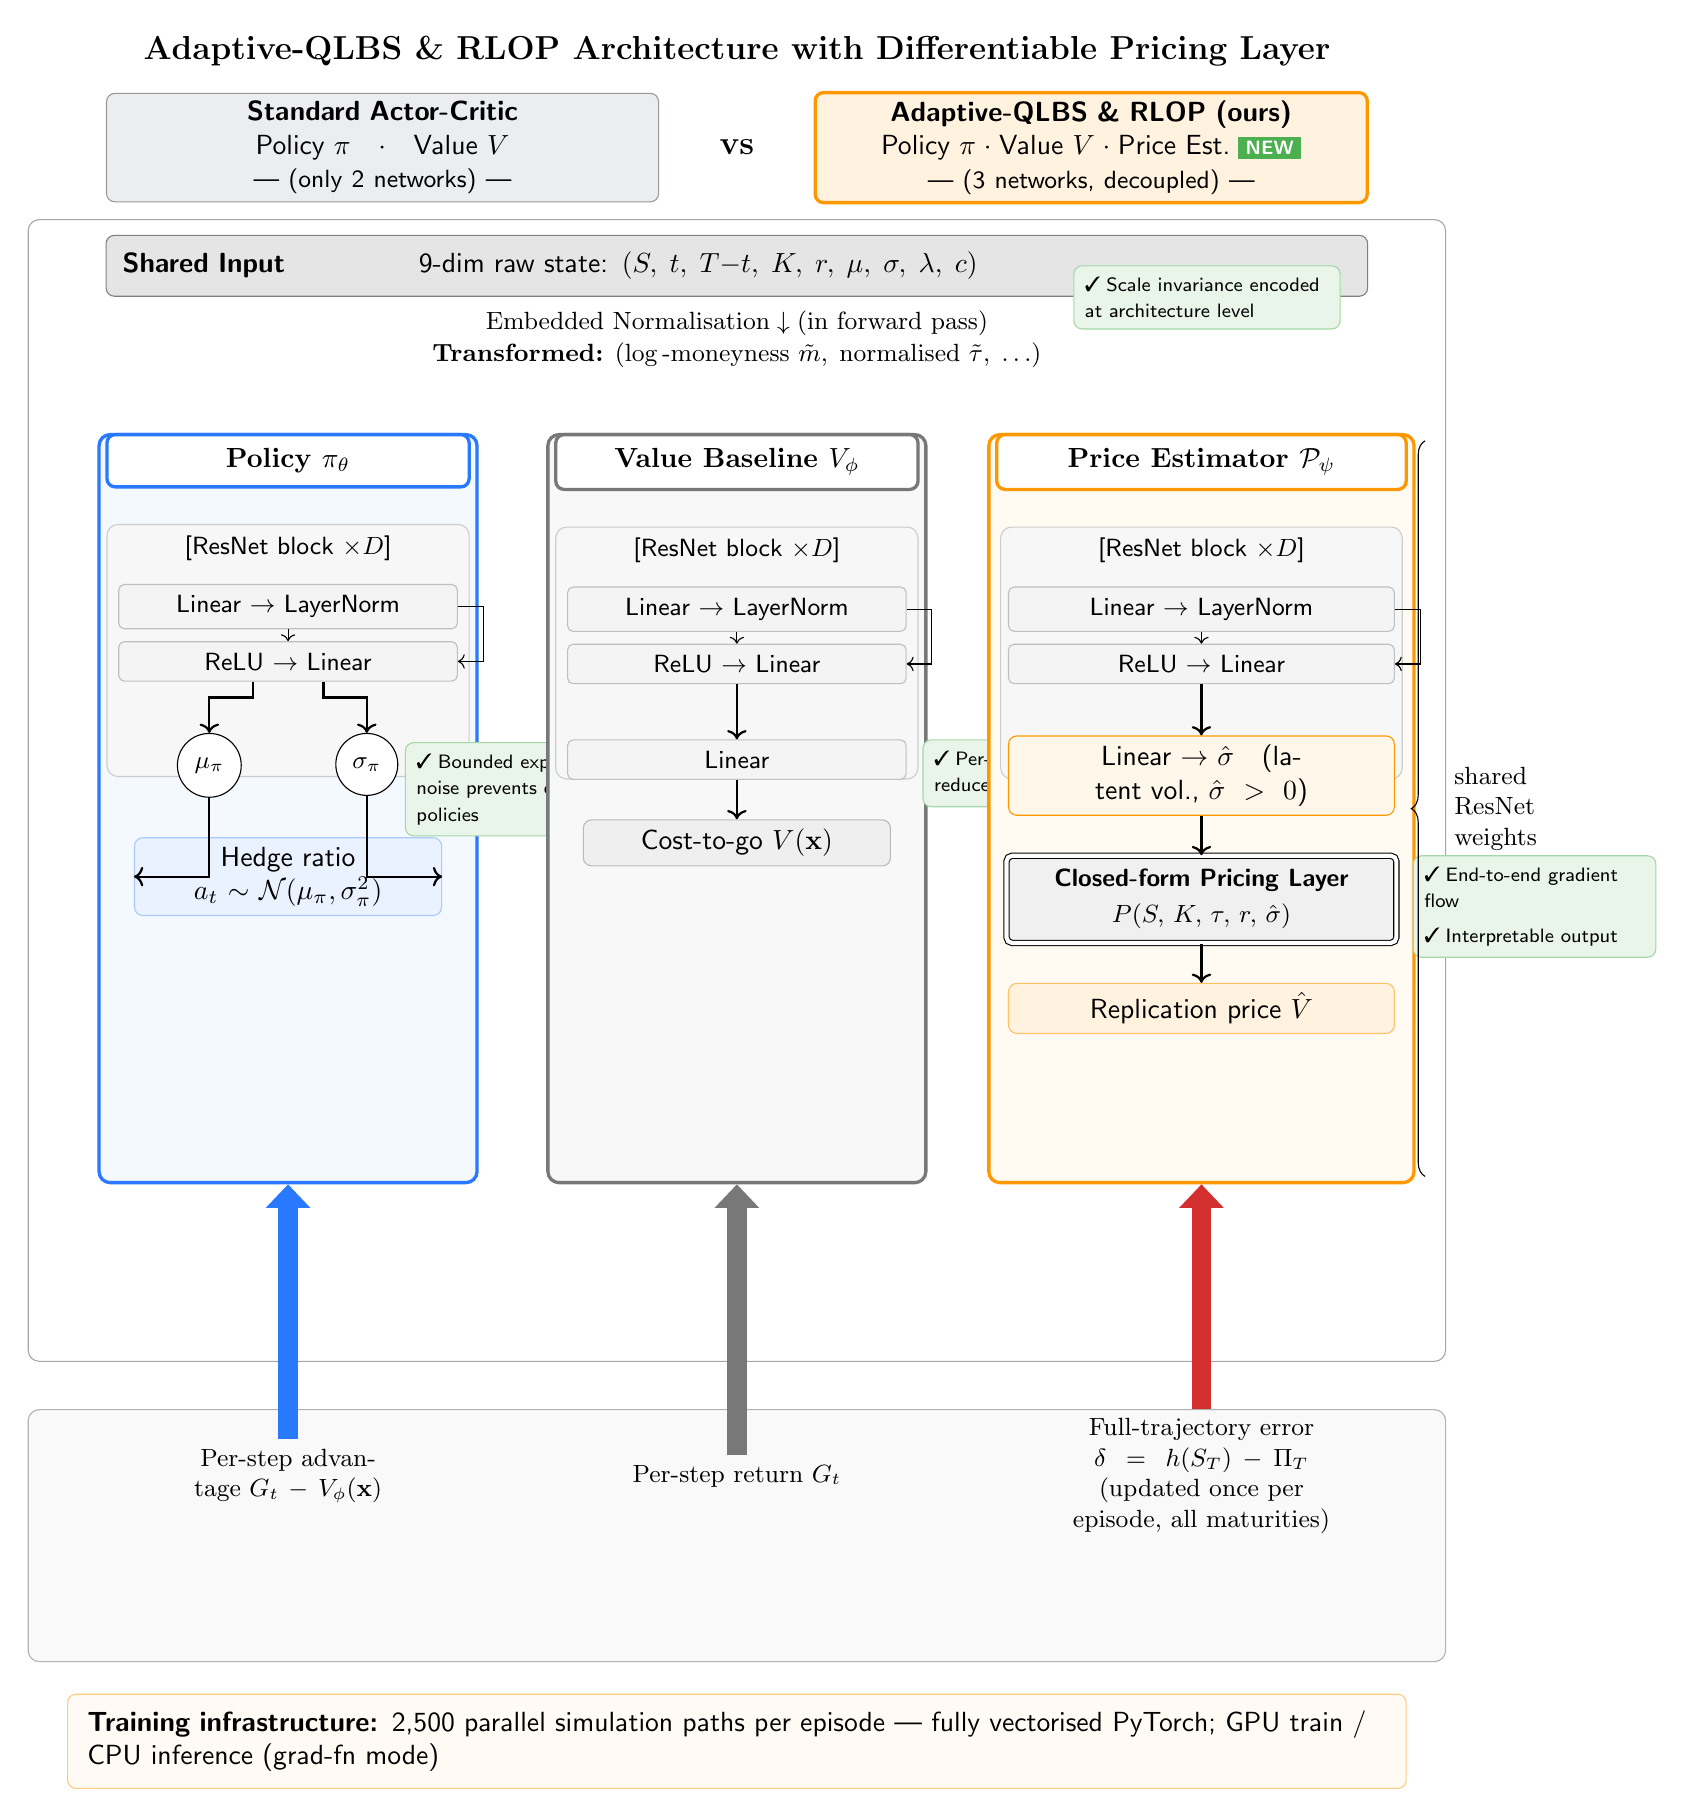
\begin{tikzpicture}[font=\sffamily]

%%====== TITLE ======
\node[font=\large\bfseries,align=center] (title)
  {Adaptive-QLBS \& RLOP Architecture with Differentiable Pricing Layer};

%%====== SECTION A ======
\node[sframe,draw=none,below=0.cm of title,minimum width=18cm,minimum height=1.8cm] (boxA) {};

\node[rectangle,rounded corners=3pt,draw=black!40,fill=colorAstd,
     text width=6.8cm,align=center,inner sep=3pt]
  at ($(boxA.center)+(-4.5cm,0)$) {
  \textbf{Standard Actor-Critic}\\
  Policy $\pi$\quad$\cdot$\quad Value $V$\\
  \small --- (only 2 networks) ---};

\node[font=\large\bfseries] at (boxA.center) {vs};

\node[rectangle,rounded corners=3pt,draw=priceOrange,line width=1.2pt,fill=colorAours,
     text width=6.8cm,align=center,inner sep=3pt]
  at ($(boxA.center)+(4.5cm,0)$) {
  \textbf{Adaptive-QLBS \& RLOP (ours)}\\
  Policy $\pi$\;$\cdot$\;Value $V$\;$\cdot$\;Price Est.\;\probadge{NEW}\\
  \small --- (3 networks, decoupled) ---};

%%====== SECTION B ======
\node[sframe,below=0.0cm of boxA,minimum width=18cm,minimum height=14.5cm] (boxB) {};

%% Shared input box
\node[rectangle,rounded corners=3pt,draw=black!50,fill=black!10,
     minimum width=16cm,text width=15.6cm,align=left,inner sep=6pt,
     anchor=north] (sinput) at ($(boxB.north)+(0,-0.2cm)$) {
  \textbf{Shared Input}\hspace{1.7cm}%
  9-dim raw state: $(S,\;t,\;T{-}t,\;K,\;r,\;\mu,\;\sigma,\;\lambda,\;c)$};

\node[below=0.05cm of sinput,font=\small,align=center] (normnode)
  {Embedded Normalisation\;$\downarrow$\;(in forward pass)};

\node[below=-0.15cm of normnode,font=\small,align=center] (transf)
  {\textbf{Transformed:} $(\log\text{-moneyness }\tilde{m},\;\text{normalised }\tilde{\tau},\;\ldots)$};

\node[callout,text width=3.1cm,anchor=north east]
  at ($(sinput.south east)+(-0.35cm,0.4cm)$) {
  \ding{51}\;Scale invariance encoded at architecture level};

%% Column top anchor
\coordinate (ctop) at ($(transf.south)+(0,-0.7cm)$);

%%--- POLICY column (blue) ---
\node[colfr=policyBlue,minimum width=4.8cm,minimum height=9.5cm,anchor=north]
  (box_p) at ($(ctop)+(-5.7cm,0)$) {};
\node[colhdr=policyBlue,minimum width=4.6cm,anchor=north]
  (hdr_p) at (box_p.north) {Policy $\pi_\theta$};

\node[rectangle,rounded corners=4pt,draw=gray!40,fill=gray!6,
     minimum width=4.6cm,minimum height=3.2cm,
     below=0.45cm of hdr_p] (rp1) {};
\node[font=\small\sffamily,inner sep=4pt,anchor=north] at (rp1.north)
  {[ResNet block $\times D$]};
\node[rblock] (rp2) at ($(rp1.north)+(0,-1.05cm)$) {Linear $\to$ LayerNorm};
\node[rblock,below=0.15cm of rp2] (rp3) {ReLU $\to$ Linear};
\draw[->] (rp2)--(rp3);
\draw[->] (rp2.east) -- ++(0.32cm,0) |- (rp3.east);

\node[circle,draw,fill=white,inner sep=4pt,font=\small,
     below=0.65cm of rp3,xshift=-1.0cm] (mu_p) {$\mu_\pi$};
\node[circle,draw,fill=white,inner sep=4pt,font=\small,
     below=0.65cm of rp3,xshift=+1.0cm] (sg_p) {$\sigma_\pi$};
\draw[->,thick] (rp3.south) ++(-0.45cm,0) -- ++(0,-0.2cm) -| (mu_p.north);
\draw[->,thick] (rp3.south) ++(+0.45cm,0) -- ++(0,-0.2cm) -| (sg_p.north);

\node[rectangle,rounded corners=3pt,draw=policyBlue!40,fill=policyBlue!10,
     minimum width=3.9cm,text width=3.6cm,align=center,
     below=0.5cm of mu_p,xshift=1.0cm] (hedge)
  {Hedge ratio $a_t\!\sim\!\mathcal{N}(\mu_\pi,\sigma_\pi^2)$};
\draw[->,thick] (mu_p.south) |- (hedge.west);
\draw[->,thick] (sg_p.south) |- (hedge.east);

\node[callout,text width=2.8cm,anchor=north west]
  at ($(sg_p.north east)+(0.2cm,0)$) {
  \ding{51}\;Bounded exploration noise prevents degenerate policies};

%%--- VALUE column (gray) ---
\node[colfr=valueGray,minimum width=4.8cm,minimum height=9.5cm,anchor=north]
  (box_v) at ($(ctop)+(0,0)$) {};
\node[colhdr=valueGray,minimum width=4.6cm,anchor=north]
  (hdr_v) at (box_v.north) {Value Baseline $V_\phi$};

\node[rectangle,rounded corners=4pt,draw=gray!40,fill=gray!6,
     minimum width=4.6cm,minimum height=3.2cm,
     below=0.45cm of hdr_v] (rv1) {};
\node[font=\small\sffamily,inner sep=4pt,anchor=north] at (rv1.north)
  {[ResNet block $\times D$]};
\node[rblock] (rv2) at ($(rv1.north)+(0,-1.05cm)$) {Linear $\to$ LayerNorm};
\node[rblock,below=0.15cm of rv2] (rv3) {ReLU $\to$ Linear};
\draw[->] (rv2)--(rv3);
\draw[->] (rv2.east) -- ++(0.32cm,0) |- (rv3.east);

\node[rblock,below=0.7cm of rv3] (lin_v) {Linear};
\draw[->,thick] (rv3)--(lin_v);

\node[rectangle,rounded corners=3pt,draw=valueGray!50,fill=valueGray!12,
     minimum width=3.9cm,below=0.5cm of lin_v] (ctg) {Cost-to-go $V(\mathbf{x})$};
\draw[->,thick] (lin_v)--(ctg);

\node[callout,text width=2.8cm,anchor=north west]
  at ($(lin_v.north east)+(0.2cm,0)$) {
  \ding{51}\;Per-step signal only --- reduces gradient variance};

%%--- PRICE column (orange, wider) ---
\node[colfr=priceOrange,minimum width=5.4cm,minimum height=9.5cm,anchor=north]
  (box_pr) at ($(ctop)+(+5.9cm,0)$) {};
\node[colhdr=priceOrange,minimum width=5.2cm,anchor=north]
  (hdr_pr) at (box_pr.north) {Price Estimator $\mathcal{P}_\psi$};

\node[rectangle,rounded corners=4pt,draw=gray!40,fill=gray!6,
     minimum width=5.1cm,minimum height=3.2cm,
     below=0.45cm of hdr_pr] (rpr1) {};
\node[font=\small\sffamily,inner sep=4pt,anchor=north] at (rpr1.north)
  {[ResNet block $\times D$]};
\node[rblockW] (rpr2) at ($(rpr1.north)+(0,-1.05cm)$) {Linear $\to$ LayerNorm};
\node[rblockW,below=0.15cm of rpr2] (rpr3) {ReLU $\to$ Linear};
\draw[->] (rpr2)--(rpr3);
\draw[->] (rpr2.east) -- ++(0.32cm,0) |- (rpr3.east);

\node[rectangle,rounded corners=3pt,draw=priceOrange,fill=colorAours!70,
     minimum width=4.9cm,text width=4.6cm,align=center,
     below=0.65cm of rpr3] (latvol)
  {Linear $\to$ $\hat{\sigma}$\quad(latent vol., $\hat{\sigma}>0$)};
\draw[->,thick] (rpr3)--(latvol);

\node[dblbox,minimum width=4.9cm,text width=4.6cm,
     below=0.5cm of latvol] (prl)
  {Closed-form Pricing Layer\\[2pt]$P(S,\,K,\,\tau,\,r,\,\hat{\sigma})$};
\draw[->,thick] (latvol)--(prl);

\node[rectangle,rounded corners=3pt,draw=priceOrange!60,fill=priceOrange!12,
     minimum width=4.9cm,below=0.5cm of prl] (rep)
  {Replication price $\hat{V}$};
\draw[->,thick] (prl)--(rep);

\node[callout,text width=2.8cm,anchor=north west]
  at ($(prl.north east)+(0.2cm,0)$) {
  \ding{51}\;End-to-end gradient flow\\[3pt]
  \ding{51}\;Interpretable output};

%%--- Shared weights brace (right side of Price box, annotating Policy+Price share) ---
\draw[decorate,decoration={brace,amplitude=5pt,mirror}]
  ($(box_pr.north east)+(0.12cm,-0.1cm)$) -- ($(box_pr.south east)+(0.12cm,0.1cm)$)
  node[midway,right=7pt,font=\small,text width=1.8cm,align=left]
  {shared\\ResNet\\weights};

%%====== SECTION C ======
\node[sframe,fill=gray!5,draw=black!30,
     below=0.6cm of boxB,minimum width=18cm,minimum height=3.2cm] (boxC) {};

\node[font=\small,align=center,text width=4.2cm]
  (lp) at ($(boxC.north)+(-5.7cm,-0.85cm)$)
  {Per-step advantage $G_t - V_\phi(\mathbf{x})$};
\draw[garrow,policyBlue]   (lp.north)  -- (box_p.south);

\node[font=\small,align=center,text width=3.5cm]
  (lv) at ($(boxC.north)+(0,-0.85cm)$)
  {Per-step return $G_t$};
\draw[garrow,valueGray]    (lv.north)  -- (box_v.south);

\node[font=\small,align=center,text width=5cm]
  (lpr) at ($(boxC.north)+(5.9cm,-0.85cm)$)
  {Full-trajectory error $\delta = h(S_T) - \Pi_T$\\
   (updated once per episode, all maturities)};
\draw[garrow,gradientRed]  (lpr.north) -- (box_pr.south);

%%====== FOOTER (outside boxC) ======
\node[rectangle,rounded corners=3pt,draw=priceOrange!50,fill=colorAours!35,
     minimum width=17cm,text width=16.5cm,align=left,inner sep=6pt,
     below=0.4cm of boxC] {
  \textbf{Training infrastructure:} 2{,}500 parallel simulation paths per episode
  --- fully vectorised PyTorch; GPU train / CPU inference (grad-fn mode)};

\end{tikzpicture}
\end{document}
